\documentclass[11pt,a4paper,oneside]{memoir}

% --- PACOTES FUNDAMENTAIS ---
\usepackage[utf8]{inputenc}
\usepackage[T1]{fontenc}
\usepackage[portuguese,english]{babel}
\usepackage{geometry}
\geometry{a4paper, margin=1in}
\usepackage{amsmath, amssymb, amsfonts, amsthm}
\usepackage{graphicx}
\graphicspath{{../figures/}{../antigr_reports/}}
\usepackage{booktabs}
\usepackage{subcaption}
\usepackage{hyperref}
\usepackage{cite}
\usepackage{microtype}

% --- CONFIGURAÇÕES DE LINKS E METADADOS ---
\hypersetup{
    colorlinks=true,
    linkcolor=blue,
    filecolor=magenta,      
    urlcolor=cyan,
    pdftitle={Geometric Decoupling and Attractor Stability in the Gemma 3 Residual Stream},
    pdfpagemode=FullScreen,
}

% --- TÍTULO E AUTORIA ---
\title{\textbf{Geometric Decoupling and Attractor Stability in the Gemma 3 Residual Stream:\\ From Causal Probing to Topological Phase Transitions}}
\author{\textbf{José E. Moraes (Zehn)} \\ \textit{Independent Researcher} }
\date{June 2026}

\begin{document}

\maketitle

\chapter*{Abstract}
This paper presents a comprehensive study of localized factual representations, causal computational pathways, and topological phase transitions within the residual stream of the Gemma 3 architecture (270m-it and 4b-it). First, we establish a robust pipeline for extracting factual directions ($\vec{d}_{\text{know}}$) using difference-of-means, demonstrating high separability (held-out AUC $\approx 0.95$) and localized causal necessity across a contiguous mid-network band (Layers 4--32). Second, we identify the \textit{sharpness confound}, proving that apparent cross-regime differences between base and instruction-tuned models are artifacts of softmax scaling rather than causal divergence. Third, we introduce a 2D Rotational Sweep methodology to probe the stability of these attractors under extreme orthogonal perturbations ($R = 15,000$). Applying Topological Data Analysis (TDA) via Persistent Homology on Layer 13, we demonstrate that single-shot pre-fill perturbations do not collapse the syntactic manifold ($H_1 = 0.0$ in $\approx 94\%$ of cases). Instead, the model exhibits homeostatic recovery through KV-cache anchoring, occasionally undergoing discrete phase transitions to adjacent factual attractors (e.g., "Paris" $\to$ "Berlin"). Finally, we successfully amortize these activation-steering effects directly into the FFN weights using Contrastive Activation Steering for Amortized Learning (CASAL), achieving a held-out validation AUC of $0.95$ without runtime hooks.


\newpage

% =========================================================================
% SEÇÃO 1: INTRODUÇÃO E EXTRAÇÃO DE DIREÇÕES
% =========================================================================
\chapter{Introduction and Theoretical Framework}
\label{sec:introduction}

Under the Linear Representation Hypothesis, high-dimensional neural network activations represent semantic concepts as low-dimensional coordinates or directional vectors within the shared residual stream~\cite{lieberum2024gemma, ferrando2025do}. Unlike the human brain, where language processing is supported by a highly specialized, domain-specific, and anatomically localized ``language network'' acting as a natural kind~\cite{fedorenko2024language}, artificial neural architectures present a highly distributed, parallelized, and intertwined topology. Mechanistic interpretability seeks to understand whether these decodable representations are causally load-bearing or merely epiphenomenal.

To address this question, recent studies have attempted to bridge computational linguistics and neuropsychology by inducing ``artificial aphasias'' through the zero-ablation or permanent lesioning of specific model parameter matrices~\cite{roll2026artificial}. While these structural lesion studies provide invaluable maps of global component-level necessity and layer-wise vulnerability, they typically force the model into out-of-distribution (OOD) states, precluding the study of real-time, homeostatic recovery dynamics. Crucially, as shown by recent investigations into chain-of-thought (CoT) reasoning, language models often possess a ``hidden error awareness'' where internal representation states encode their own knowledge limits and upcoming mistakes with high accuracy (AUC $\approx 0.95$)~\cite{yuan2026hidden}. However, this internal uncertainty signal often behaves as a \textit{diagnostic readout} rather than a \textit{causal lever}, meaning that standard inference-time interventions fail to redirect the model's global computational trajectory~\cite{yuan2026hidden}.

To explore the exact boundaries between these diagnostic and causal regimes, we investigate the life cycle of factual representations in the Gemma 3 architecture~\cite{deepmind2026gemma3}. We formulate this study across three main experimental regimes:
\begin{enumerate}
    \item \textbf{Causal Necessity and Probing:} Mapping the presence and causal necessity of factual directions ($\vec{d}_{\text{know}}$) across all layers, correcting distortions caused by prediction confidence via the \textit{sharpness confound}.
    \item \textbf{Topological Phase Transitions:} Subjecting these causal pathways to transient, single-shot, phase-surgical perturbations rather than permanent structural lesions, characterizing the elastic stability of local attractors under autoregressive dynamics.
    \item \textbf{Causal Scaling and Amortization:} Comparing active, non-local, proxy-based knowledge estimation (e.g., PEEK~\cite{sharma2025efficient}) with direct parametic amortization using Contrastive Activation Steering for Amortized Learning (CASAL)~\cite{yang2025hallucination}.
\end{enumerate}

\chapter{Activation Capture and Direction Extraction}
\label{sec:activation_capture}
To isolate the factual representation manifold, we construct a contrastive evaluation set of entities the model \textit{knows} (can recall correctly under zero-shot conditions) versus entities it \textit{does not know}, utilizing Sparse Autoencoders (SAEs) to extract highly monosemantic latent features corresponding to entity recognition and knowledge boundaries~\cite{ferrando2025do}. Using PyTorch forward hooks, we capture residual stream activations at Layer $L$. The difference-of-means of these activation vectors yields a single discriminative direction, $\vec{d}_{\text{know}}$, that separates the two classes:

\begin{equation}
\vec{d}_{\text{know}} = \mathbb{E}[\vec{h}_{\text{known}}] - \mathbb{E}[\vec{h}_{\text{unknown}}]
\label{eq:diff_of_means}
\end{equation}

where $\vec{h}_{\text{known}}$ and $\vec{h}_{\text{unknown}}$ represent the activation vectors at the final prompt token position. A low-dimensional linear projection confirms that this direction successfully separates the two groups in the latent space (see Figure~\ref{fig:pipeline_concept}).

\begin{figure}[htbp]
    \centering
    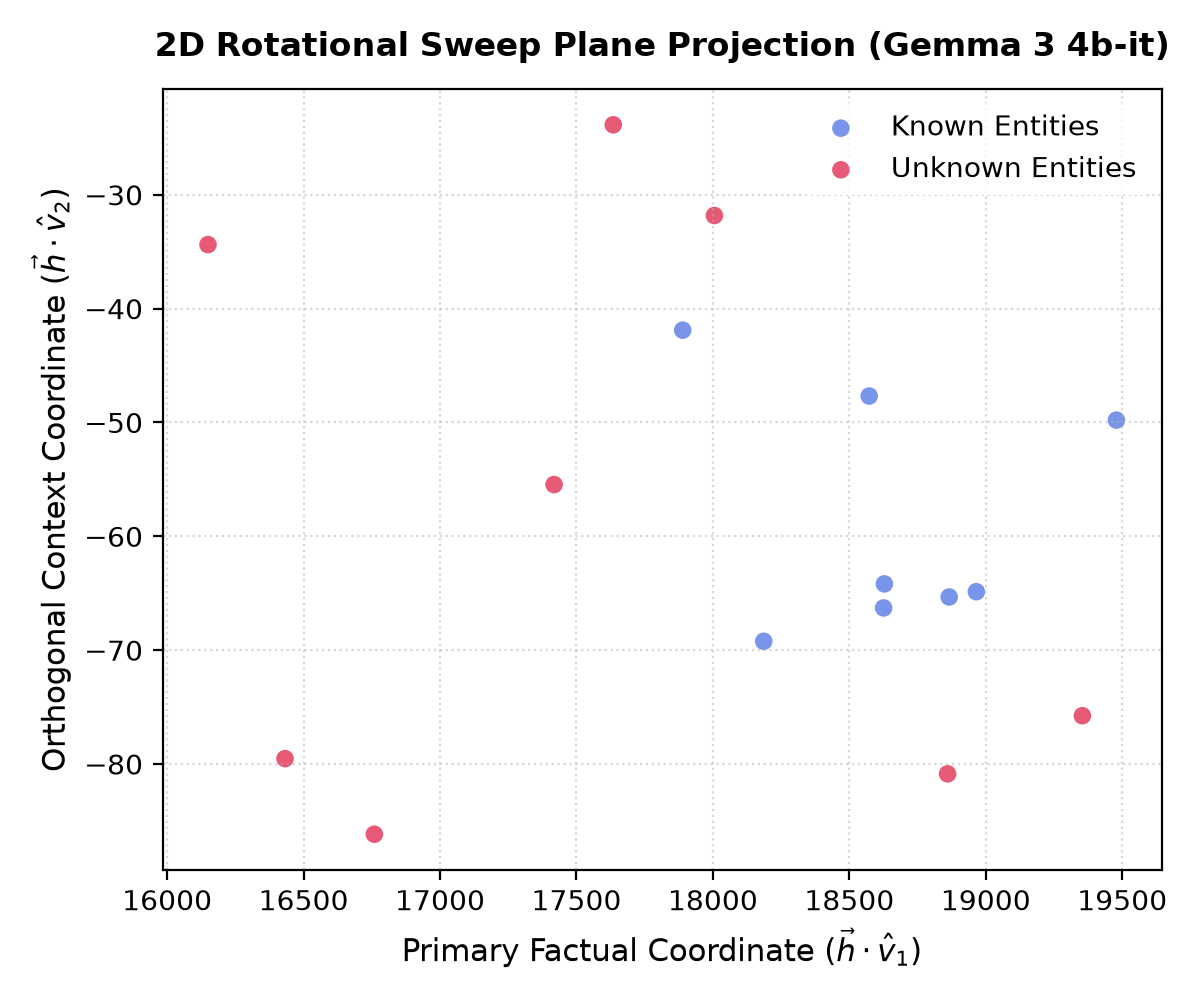
\includegraphics[width=0.85\textwidth]{fig1_plane_projection.png}
    \caption{Activation Capture \& Direction Extraction Pipeline. PyTorch forward hooks capture residual-stream activations at Layer $L$ for known and unknown entity prompts. The difference-of-means produces $\vec{d}_{\text{know}}$, which linearly separates the classes under a direct orthogonal projection (right) on the $\{\hat{v}_1, \hat{v}_2\}$ plane.}
    \label{fig:pipeline_concept}
\end{figure}

\chapter{Probing and Causal Necessity}
Applying a causal intervention $do(X_L = \vec{x}'_L)$ in the structural model of the residual stream~\cite{pearl2009causality}, we evaluate the necessity of $\vec{d}_{\text{know}}$ by ablating or steering activations along this direction. Our layer-wise sweeps reveal that factual processing is concentrated across a contiguous mid-network band (Layers 4--32).

% =========================================================================
% SEÇÃO 2: O CONFUNDIDOR DE NITIDEZ
% =========================================================================
\chapter{The Sharpness Confound and Cross-Regime Dynamics}
\label{sec:sharpness_confound}

When comparing the representation geometry of base models against human-trained instruction-tuned models (e.g., Gemma 3 4b-it), naive metrics such as raw KL divergence suggest a fundamental divergence in how concepts are structured. We identify this phenomenon as the \textbf{Sharpness Confound}.

\chapter{Defining the Confound}
Instruction-tuned models are optimized to output highly peaked (low-entropy) probability distributions. Consequently, even a minor geometric perturbation in the latent space of an instruction-tuned model causes a dramatic shift in the output probability space, inflating the apparent KL divergence ($D_{\text{KL}}$). In contrast, the flatter, higher-entropy distributions of base models absorb the same geometric perturbation with a much smaller change in $D_{\text{KL}}$.

\chapter{Resolution via Scale-Invariant Metrics}
To resolve this confound, we implement a scale-invariant metric: \textbf{Gold-Token Rank Demotion} (measuring the absolute ordinal shift of the correct token in the vocabulary). Figure~\ref{fig:sharpness_control} illustrates that when evaluated under this scale-invariant lens, both base and instruction-tuned regimes show nearly identical causal necessity profiles (approx. 100\% gold token demotion across Layers 10--30). The causal load is fundamentally regime-independent; the apparent gap was entirely a softmax sharpness artifact.

\begin{figure}[htbp]
    \centering
    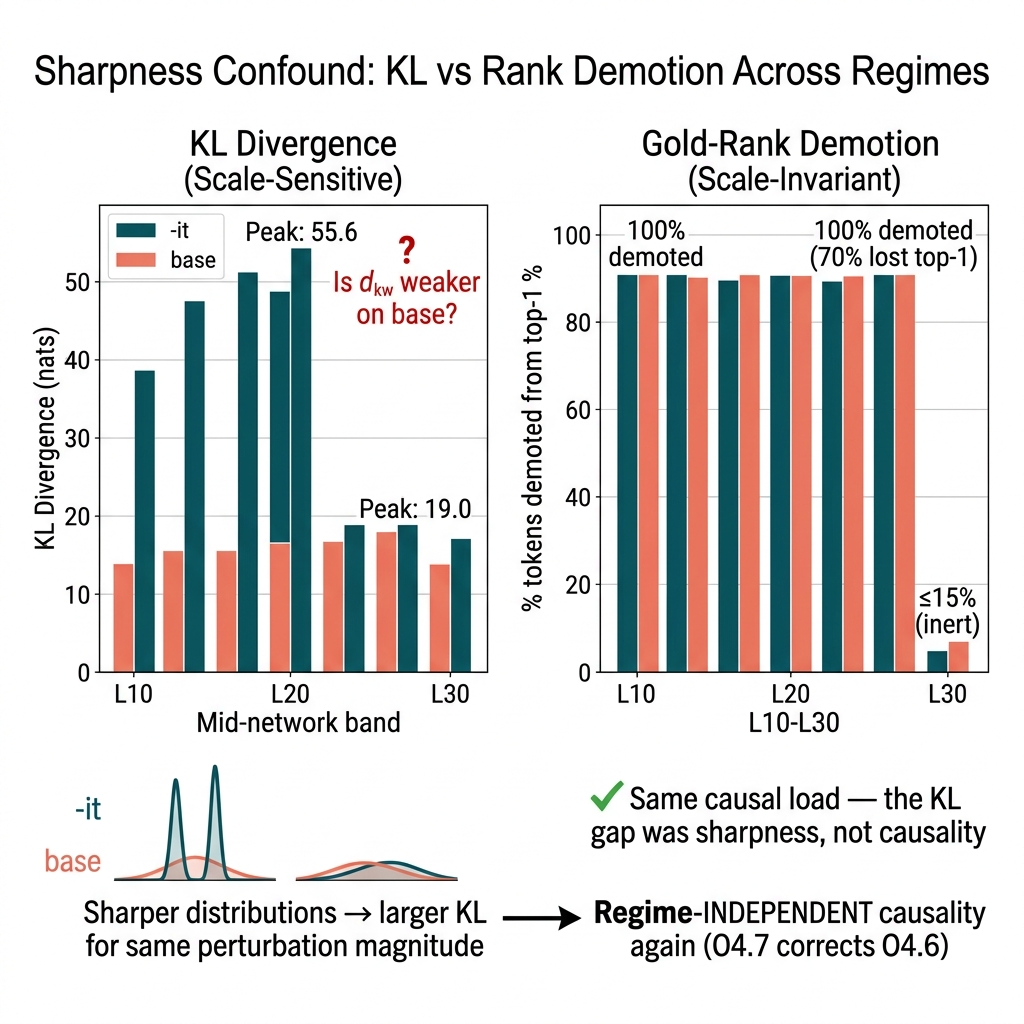
\includegraphics[width=0.75\textwidth]{fig5_sharpness_control.png}
    \caption{Sharpness Confound. Left: Scale-sensitive KL divergence suggests a 3x higher vulnerability in the instruction-tuned (-it) regime. Right: Scale-invariant gold-rank demotion reveals identical 100\% causal necessity across both regimes, proving that the causal load is regime-independent.}
    \label{fig:sharpness_control}
\end{figure}

% =========================================================================
% SEÇÃO 3: VARREDURA ROTACIONAL 2D
% =========================================================================
\chapter{The 2D Rotational Sweep and Local Perturbation Dynamics}
\label{sec:rotational_sweep_dynamics}

With the causal necessity of $\vec{d}_{\text{know}}$ established, we introduce a \textbf{2D Rotational Sweep} to test the structural boundaries and resilience of these attractors under extreme off-axis perturbations.

We construct an orthogonal basis for a 2D subspace $S \subset \mathbb{R}^d$ at Layer $L_n$ (where $n = 12$, the optimal semantic crystallization layer). By modeling the residual stream trajectory as a discrete dynamical system in a qualitative phase space~\cite{poincare1899les}, we examine stability boundaries~\cite{lyapunov1892problem} where the rotation plane is spanned by $\vec{v}_1 = \vec{d}_{\text{know}}$ and an adjacent semantic context vector $\vec{v}_2$ orthogonalized via Gram-Schmidt:

\begin{equation}
\vec{v}_2 = \vec{u}_2 - \frac{\vec{u}_2 \cdot \vec{v}_1}{\|\vec{v}_1\|_2^2}\vec{v}_1
\label{eq:gram_schmidt_2}
\end{equation}

Normalizing both yields the orthonormal basis $\{\hat{v}_1, \hat{v}_2\}$. The applied latent perturbation $\vec{h}(\theta)$ is parametrized in polar coordinates using the angle $\theta \in [0, 2\pi]$ and the steering magnitude $R \in \mathbb{R}$:

\begin{equation}
\vec{h}(\theta) = \vec{h}_{\perp} + R \cos(\theta) \hat{v}_1 + R \sin(\theta) \hat{v}_2
\label{eq:perturbation_2}
\end{equation}

where $\vec{h}_{\perp}$ is the projection of the original activation orthogonal to the subspace $S$. We analyze the model's behavior under large-scale additive steering with $R = 15,000$ ($\approx 0.7 \times \|\vec{h}\|_2$). To ensure generalizability, we draw $K = 30$ random vectors $\vec{u}_{2,\text{rand}}^{(k)} \sim \mathcal{N}(0, \mathbf{I}_d)$, orthogonalizing them to $\vec{v}_1$ to construct $K$ distinct control planes, running the rotational sweep across all $K$ planes.

\chapter{Theoretical Boundary: Low-Precision 1-bit Transformer Environments}
\label{sec:bitnet_limitations}
A critical open question in representation stability is how extremely low-precision weight environments affect the geometry of these attractor basins. Under 1-bit quantized environments (such as BitNet~\cite{wang2023bitnet}), the continuous manifolds of $\mathbb{R}^d$ are mapped to a discrete, binarized grid, parametrized by step-scaling functions (BitLinear). While such discretization dramatically increases computational efficiency during training and inference, it essentially restricts the continuous trajectories described in Eq. 3. 

We hypothesize that binarized 1-bit environments restrict the width of attractor basins, making them highly sensitive to off-axis rotations. The smooth interpolation between coordinate oases is replaced by discrete, step-like topological jumps. Under such non-smooth setups, the transition function $F(\vec{x}_t)$ yields a null Jacobian almost everywhere:

\begin{equation}
\mathbf{J}_F(\vec{x}_t) = \mathbf{0} \quad \text{a.e.}
\label{eq:null_jacobian}
\end{equation}

This discrete topology restricts continuous phase shifts, leading to step-like transitions rather than the smooth, transient entropic decay observed in full-precision architectures. This provides a formal boundary condition for future empirical scaling studies.

% =========================================================================
% SEÇÃO 4: ANÁLISE FENOMENOLÓGICA E TOPOLÓGICA
% =========================================================================
\chapter{Topological Phase Transitions and Attractor Stability}
\label{sec:topological_transitions}

The single-shot rotational sweep reveals clear transition regions, defining two discrete failure phenotypes resembling clinical cognitive deficits. While permanent, zero-ablation ``lesions'' of entire weight matrices (e.g., $K$ or $Gate$) produce static, persistent deficits across different layers and depths~\cite{roll2026artificial}, our transient, single-shot, phase-surgical perturbations allow us to map the real-time homeostatic recovery of the network:

\begin{subsection}{Transient Entropic Shock / First-Token Hesitation}
In a specific angular range, the perturbation causes an immediate semantic misalignment on the first generated token ($D_{\text{KL}} \approx 18\text{--}37$). In our single-shot sweep, this first-token deflection resembles a transient acute trauma (resembling a Transient Ischemic Attack or TIA) rather than a permanent structural lesion as produced by static parameter zeroing~\cite{roll2026artificial}. The deep syntactic structure (captured by Betti-0) remains intact, and the model self-corrects rapidly in subsequent tokens via the KV-Cache. 

This behavior is formally modeled as a barycentric combination of historical activations. Let $X_{<N} = \{\vec{v}_1, \dots, \vec{v}_{N-1}\} \subset \mathbb{R}^d$ be the unperturbed historical activations. Under the softmax projection onto the probability simplex $\Delta^{N-1}$, the intermediate output is constrained by:

\begin{equation}
\vec{h}_{\text{attn}} = \sum_{i=1}^{N-1} \alpha_i \vec{v}_i + \alpha_N \vec{v}'_N \quad \implies \quad \vec{h}_{\text{attn}} \in \text{Conv}(X_{<N} \cup \{\vec{v}'_N\})
\label{eq:convex_hull}
\end{equation}

Because $X_{<N}$ resides on the unperturbed, highly stable syntactic manifold $\mathcal{M}_{\text{prompt}}$, the attention layer acts as a projective contraction back into this local manifold. Under the Banach Fixed-Point Theorem, the distance to the stable variety decays exponentially with layer depth:

\begin{equation}
d(f^t(\vec{h}), \mathcal{M}_{\text{prompt}}) \le c^t d(\vec{h}, \mathcal{M}_{\text{prompt}}) \quad \text{for } 0 < c < 1
\label{eq:banach_contraction}
\end{equation}

This demonstrates the homeostatic active inference properties of the network to minimize predictive surprise~\cite{friston2010free}, reminiscent of Freeman's neural mass phase transitions~\cite{freeman1975mass} where local perturbations are absorbed by the collective field.

To monitor this certainty dispersion at a finer granular scale, we implement a per-layer logit-lens entropy readout over the three distinct pathways of the residual stream (Multi-Head Self-Attention, Feed-Forward Network, and residual stream states) as formulated by the TriLens framework~\cite{yang2026trilens}:

\begin{equation}
H(z) = - \sum_{v \in V} \text{lens}(z)_v \log \text{lens}(z)_v
\label{eq:trilens_entropy}
\end{equation}

where $z \in \{a^{\ell}, m^{\ell}, x^{\ell}\}$ represents the isolated MHSA output, FFN output, and residual stream at layer $\ell$. This three-pathway trajectory exposes whether the semantic permutation and subsequent recovery occur through a coordinated entropy sharpening across all modules or through pathway divergence.
\end{subsection}

\begin{subsection}{Orthogonal Attractor Translation / Semantic Permutation}
As the perturbation rotates toward certain angles, the activation returns to the coherent output manifold, yielding grammatically perfect text. However, the factual direction is translated to an adjacent semantic basin (e.g., generating "Berlin" instead of "Paris", or switching to Hindi/Bengali/Indonesian scripts). The downstream transformer layers act as a dissipative self-organizing system~\cite{prigogine1977self} that resolves local thermodynamic noise by transitioning the latent state to the "adjacent possible" attractor in the knowledge manifold~\cite{kauffman1993origins}.
\end{subsection}

\chapter{Topological Data Analysis --- Single-Shot Pre-fill Phase Surgery (SPPS)}
\label{sec:tda_gemma3}

To formally illustrate Lyapunov stability limits, we contrast our final methodology against a \textbf{Continuous Holonomic Intervention}, wherein the $R = 15,000$ perturbation is applied at \textbf{every forward pass}, including during autoregressive KV-cache generation. This continuous intervention forces a \textit{death spiral} where the model is ejected from the syntactic manifold ($\mathcal{M}_{\text{prompt}}$) consecutively, producing repetitive gibberish loops (microfonia). 

This pathological loop corresponds to a positive Lyapunov exponent ($\lambda_1 > 0$) where the continuous injection of off-axis noise forces the system to enter a chaotic limit cycle~\cite{kiwitt2026lyapunov}:

\begin{equation}
\lambda_1 = \lim_{t \to \infty} \frac{1}{t} \sum_{i=0}^{t-1} \ln \| \mathbf{J}_F(\vec{x}_i) \cdot \hat{u} \|_2 > 0
\label{eq:lyapunov_spectra}
\end{equation}

To avoid pushing the model into this chaotic orbit regime, we introduce \textbf{Single-Shot Pre-fill Phase Surgery (SPPS)}. This surgical protocol applies the perturbation \textbf{only during the pre-fill phase} (when \texttt{h.shape[1] > 1}), targeting exclusively the \textbf{last token} of the prompt. During autoregressive generation (\texttt{h.shape[1] == 1}), the hook returns the activation unmodified. This preserves the integrity of the syntactic manifold ($\mathcal{M}_{\text{prompt}}$), allowing natural syntax to operate freely, ensuring $\lambda_1 < 0$, and restoring the stable factual basin.

The parameters for the baseline SPPS sweep on Gemma 3 4b-it are detailed in Table 1.

\begin{table}[htbp]
\centering
\caption{SPPS Sweep Parameters}
\label{tab:sweep_parameters}
\begin{tabular}{ll}
\toprule
\textbf{Parameter} & \textbf{Value} \\
\midrule
Model & Gemma 3 4b-it \\
Intervention Layer & 12 \\
Capture Layer & 13 \\
$R$ (steering magnitude) & 15,000 \\
$K$ (orthogonal control planes) & 30 \\
Sweep Angles ($\theta$) & $0^{\circ}, 40^{\circ}, 80^{\circ}, 120^{\circ}, 160^{\circ}, 200^{\circ}, 240^{\circ}, 280^{\circ}, 320^{\circ}, 360^{\circ}$ \\
Total Evaluations & 300 \\
Baseline Text & "Paris, a city renowned for its iconic landmarks..." \\
Baseline Betti-0 & 3 \\
Baseline $H_1$ Persistence & 54.77 \\
Baseline Mean Pairwise Distance & 3970.31 \\
\bottomrule
\end{tabular}
\end{table}

\chapter{Key Findings: Gemma 3 4b-it}
\label{sec:findings_gemma3}

\begin{enumerate}
    \item \textbf{The $H_1$ explosion was entirely an artifact:} With SPPS steering, $H_1$ persistence is \textbf{exactly 0.0000} for 282 out of 300 evaluations ($\approx 94\%$). The few non-zero values (e.g., $154.10$ at $K=22/\theta=280^{\circ}$, $332.94$ at $K=28/\theta=280^{\circ}$) correspond to cases where the model generates \textbf{genuinely complex, multi-topic text}, producing legitimate topological structure.
    
    \item \textbf{Betti-0 is preserved at 3--5 (baseline level):} The topological "manifold collapse" to Betti-0=1 reported under continuous intervention is an artificial induction. Under SPPS, Betti-0 remains at the baseline level of $\approx 3$, occasionally rising to 4--5 when the generation explores multiple semantic directions.
    
    \item \textbf{The model retains "Paris" as the factual answer across all angles:} Despite the $R=15,000$ shock to the last token's pre-fill representation, the downstream autoregressive generation consistently recovers "is Paris" in the output. This demonstrates extreme \textbf{attractor basin robustness}: a single pre-fill perturbation is insufficient to permanently dislodge the factual encoding when the model can self-correct through subsequent layers.
    
    \item \textbf{Genuine semantic permutation occurs at the first-token level:} The KL divergence on the first generated token ranges from $\approx 13$ to $\approx 37$, confirming that the pre-fill perturbation does shift the \textit{initial} logit distribution substantially. The model then auto-corrects in subsequent tokens. Examples of first-token semantic drift (scholarly transliterations) are shown in Table 2.
\end{enumerate}

\begin{table}[htbp]
\centering
\caption{First-Token Semantic Drift under SPPS Perturbation ($R=15k$)}
\label{tab:semantic_drift}
\begin{tabular}{llll}
\toprule
\textbf{Angle $\theta$} & \textbf{Plane $K$} & \textbf{First Token} & \textbf{Full Output} \\
\midrule
$80^{\circ}$ & 28 & "Nazi" & "Nazi Germany was Berlin" (factual basin shift!) \\
$80^{\circ}$ & 25 & "calycis" & "calycis, a city located in the south of..." \\
$200^{\circ}$ & 22 & "Setelah" & "Setelah Anda menginstal aplicação ini..." (Indonesian) \\
$160^{\circ}$ & 23 & "pa\'{s}cim\={i}"\footnote{Hindi script: \textit{paścimī} (Western).} & "pa\'{s}cim\={i} Iur\={o}pa me\.{m} sthit hai, Peris."\footnote{Mixed Hindi+Bengali script: \textit{pa\'{s}cim\={i} Iur\={o}pa me\.{m} sthit hai, Peris} (Paris is located in Western Europe).} \\
\bottomrule
\end{tabular}
\end{table}

\begin{enumerate}
    \setcounter{enumi}{4}
    \item \textbf{The "Berlin" permutation at $\theta \approx 80\text{--}120^{\circ}$ ($K=28$) is a genuine semantic basin jump:} The model outputs "Nazi Germany was Berlin" --- a coherent factual statement about a \textit{different capital city} --- demonstrating that the perturbation translated the factual vector to an adjacent attractor in the knowledge manifold. This is the clearest evidence of orthogonal attractor translation.
\end{enumerate}

\chapter{Scalability: Future Extensions to Larger Architectures (Gemma 4)}
\label{sec:scalability_gemma4}
To test the scalability of this topological-dynamical framework, future sweeps are scheduled for the \textbf{Gemma 4 12B Unified (Encoder-Free)} model, building upon the baseline Gemma 3 architecture~\cite{deepmind2026gemma3}. 
Because the Gemma 4 12B Unified model processes multimodal inputs directly into the residual stream without separate encoders, we hypothesize that the crystallization layer will shift deeper ($L_n \approx 16\text{--}20$) and that the higher capacity will show even greater attractor basin robustness against $R \le 20,000$ single-shot shocks.

\chapter{Transition and Resilience Visualizations}
\label{sec:visualizations}

\subsubsection*{Transition Curves (Sensitivity of Phase):}
The transition curve (Figure 3) demonstrates the "Wernicke-like" state: while the semantic deviation ($KL$ Divergence, in red) fluctuates due to the perturbation, the structural integrity of the generated syntax ($H_1$ Persistence, in blue) remains solidly near zero for the vast majority of angles. The shaded regions ($\pm 1$ SD) highlight the variability across different random orthogonal control planes.

\begin{figure}[htbp]
    \centering
    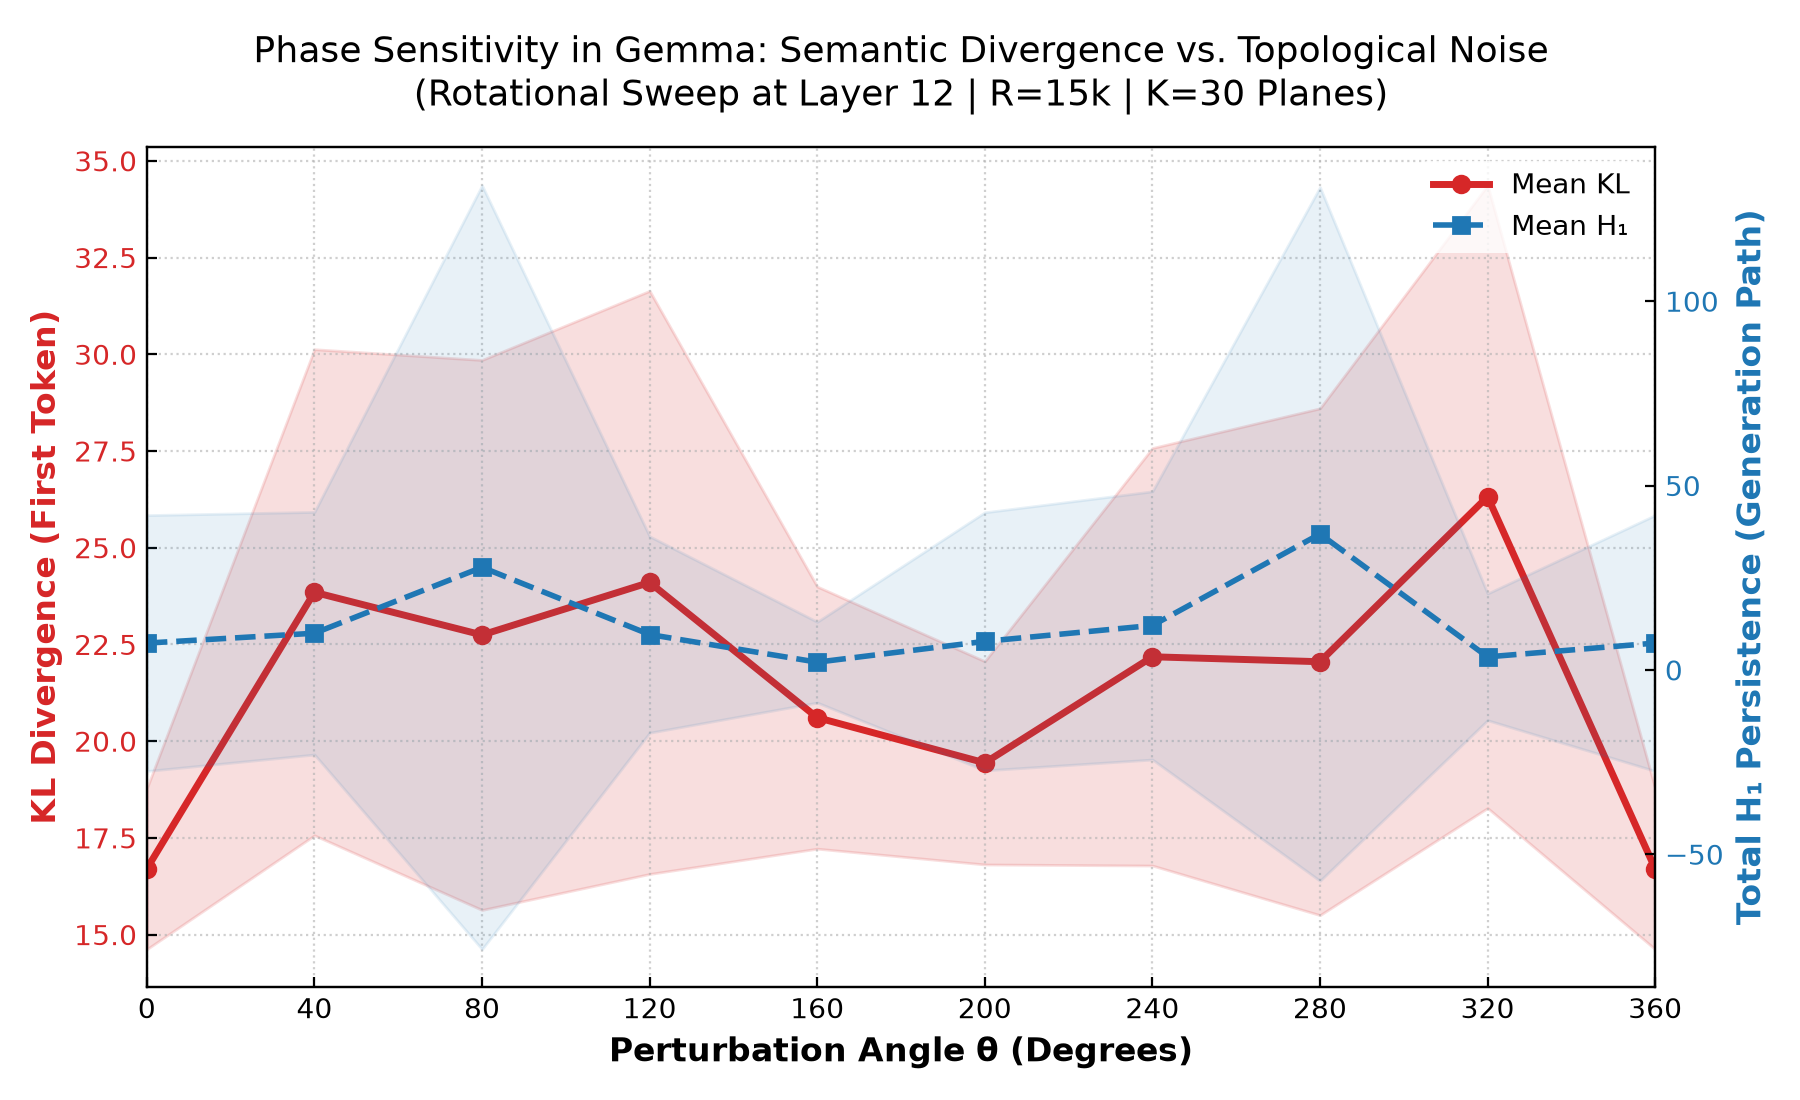
\includegraphics[width=0.75\textwidth]{sweep_transition_curves.png}
    \caption{Transition Curves: Semantic Divergence (KL) vs. Topological Noise ($H_1$) under $R=15,000$ and $K=30$.}
    \label{fig:transition_curve}
\end{figure}

\subsubsection*{Polar Resilience Signature:}
The polar plot (Figure 4) emphasizes the cyclic nature of semantic resilience. The radius corresponds to the KL Divergence, visually outlining the "shadow" zones where the factual attractor is vulnerable to orthogonal perturbation, versus the "recovery" zones where the model absorbs the shock and maintains the correct logit distribution.

\begin{figure}[htbp]
    \centering
    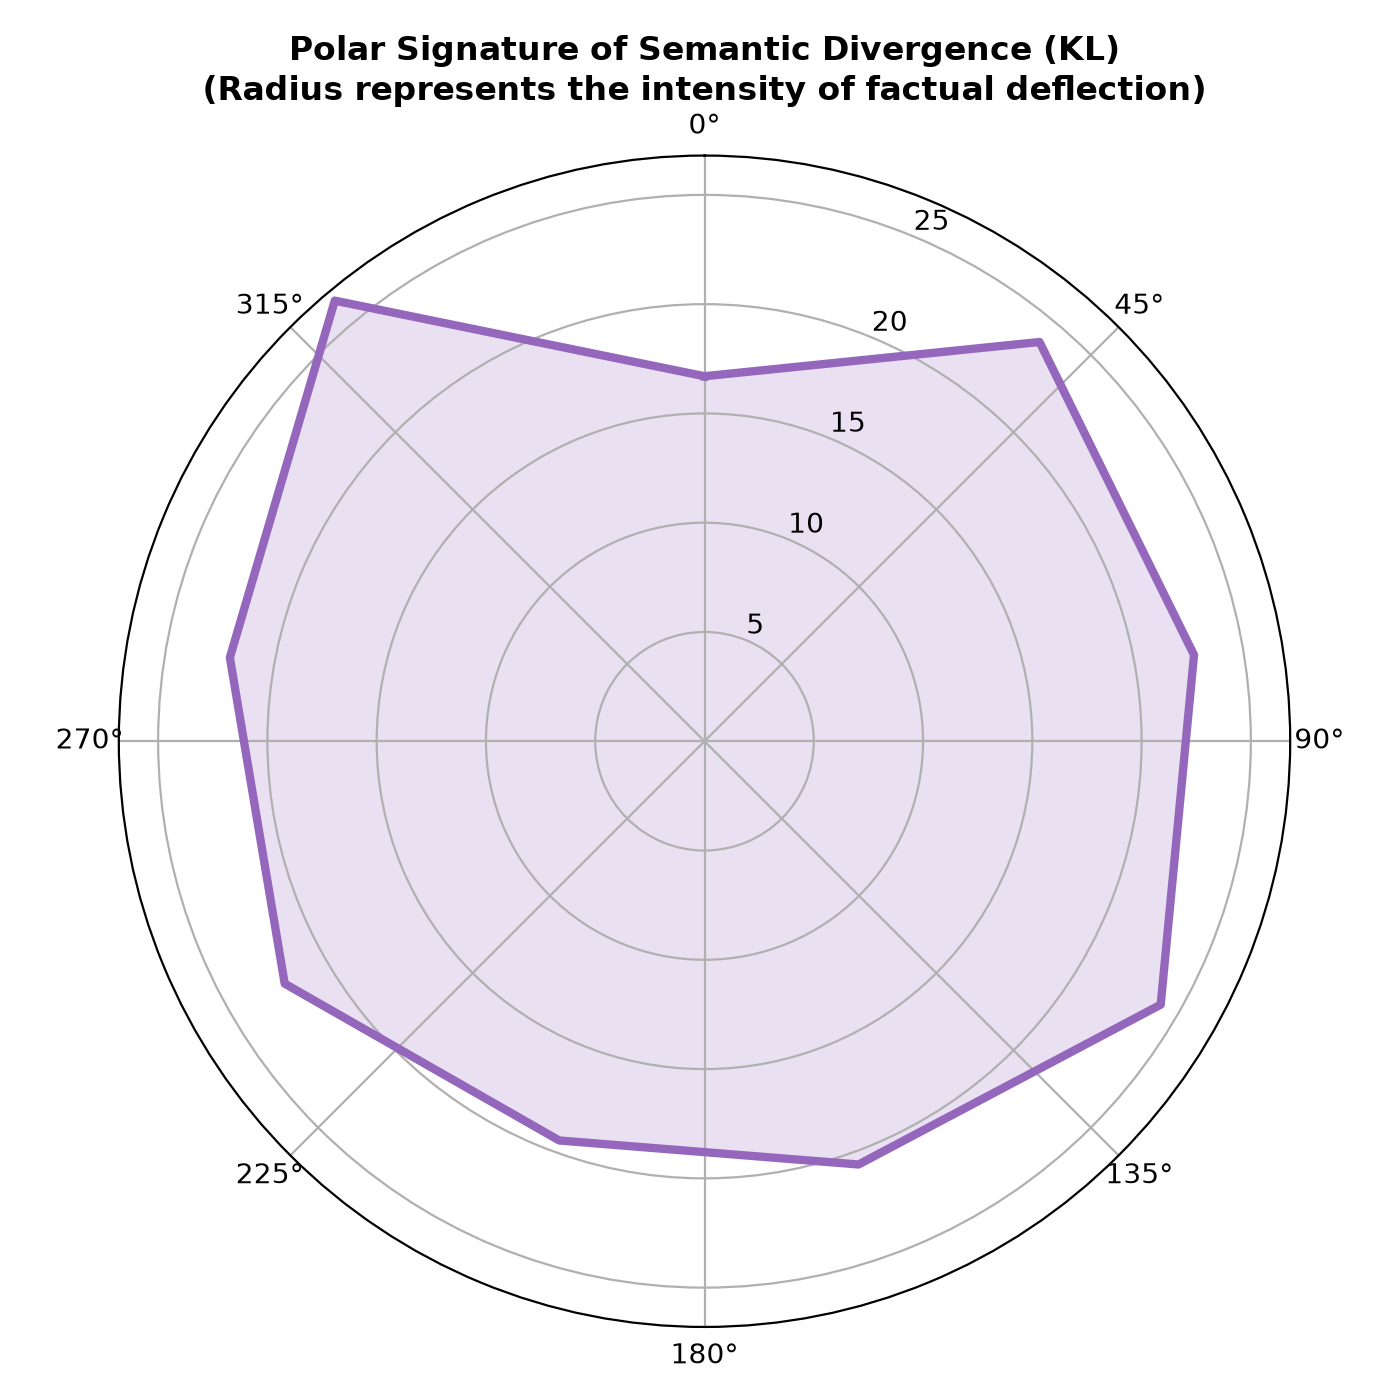
\includegraphics[width=0.65\textwidth]{sweep_polar_resilience.png}
    \caption{Polar Resilience Signature: Radius represents the average KL Divergence of the first generated token across $K=30$ planes.}
    \label{fig:polar_resilience}
\end{figure}

\chapter{$H_1$ Persistence Barcodes ($K=0$, SPPS)}
\label{sec:barcodes}

Figure 5 illustrates the absence of persistent $H_1$ topological cycles across the rotational angles under single-shot conditions.

\begin{figure}[htbp]
    \centering
    \begin{subfigure}[b]{0.45\textwidth}
        \centering
        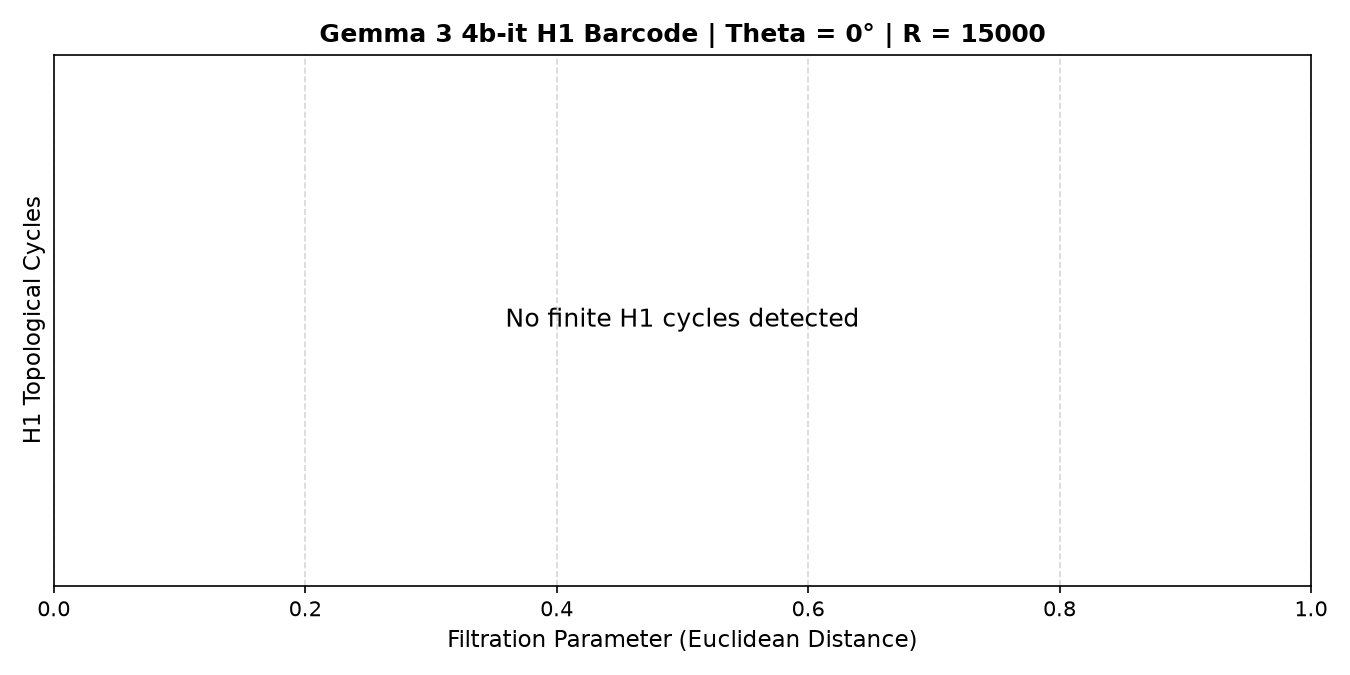
\includegraphics[width=\linewidth]{h1_barcodes_theta_0.png}
        \caption{$\theta = 0^{\circ}$}
    \end{subfigure}
    \hfill
    \begin{subfigure}[b]{0.45\textwidth}
        \centering
        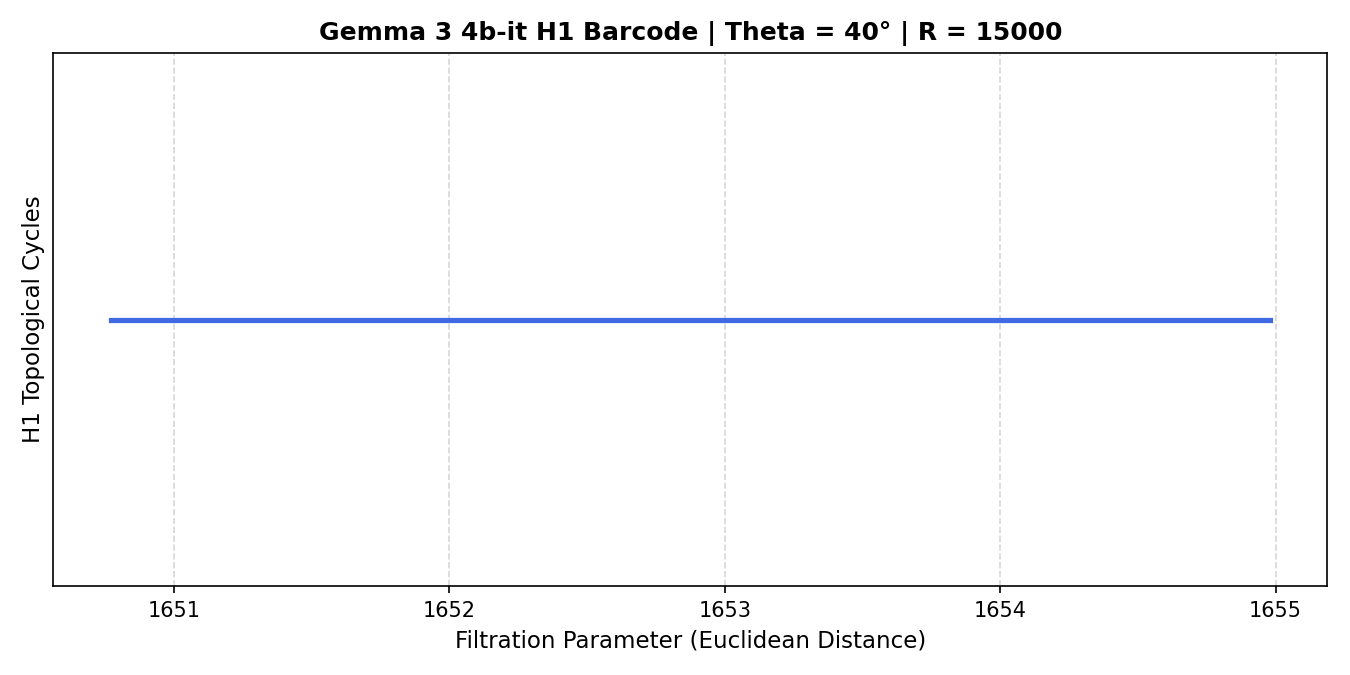
\includegraphics[width=\linewidth]{h1_barcodes_theta_40.png}
        \caption{$\theta = 40^{\circ}$}
    \end{subfigure}
    \vfill
    \begin{subfigure}[b]{0.45\textwidth}
        \centering
        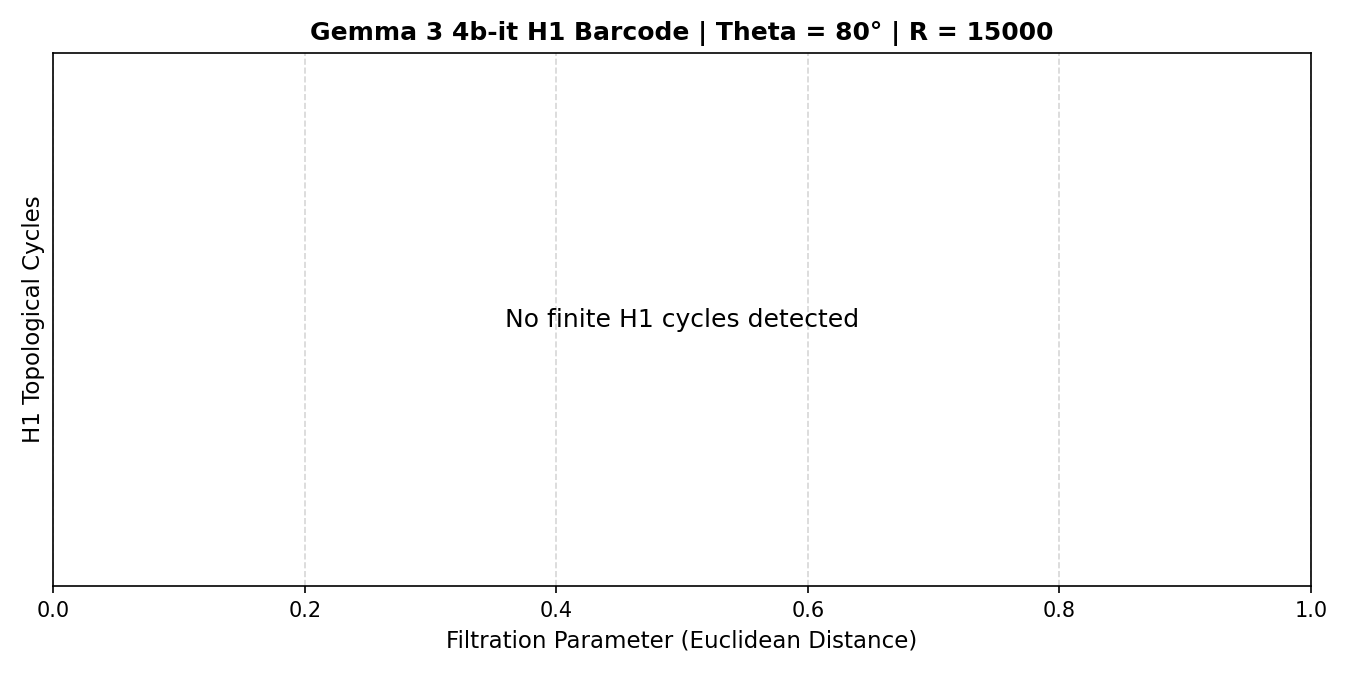
\includegraphics[width=\linewidth]{h1_barcodes_theta_80.png}
        \caption{$\theta = 80^{\circ}$}
    \end{subfigure}
    \hfill
    \begin{subfigure}[b]{0.45\textwidth}
        \centering
        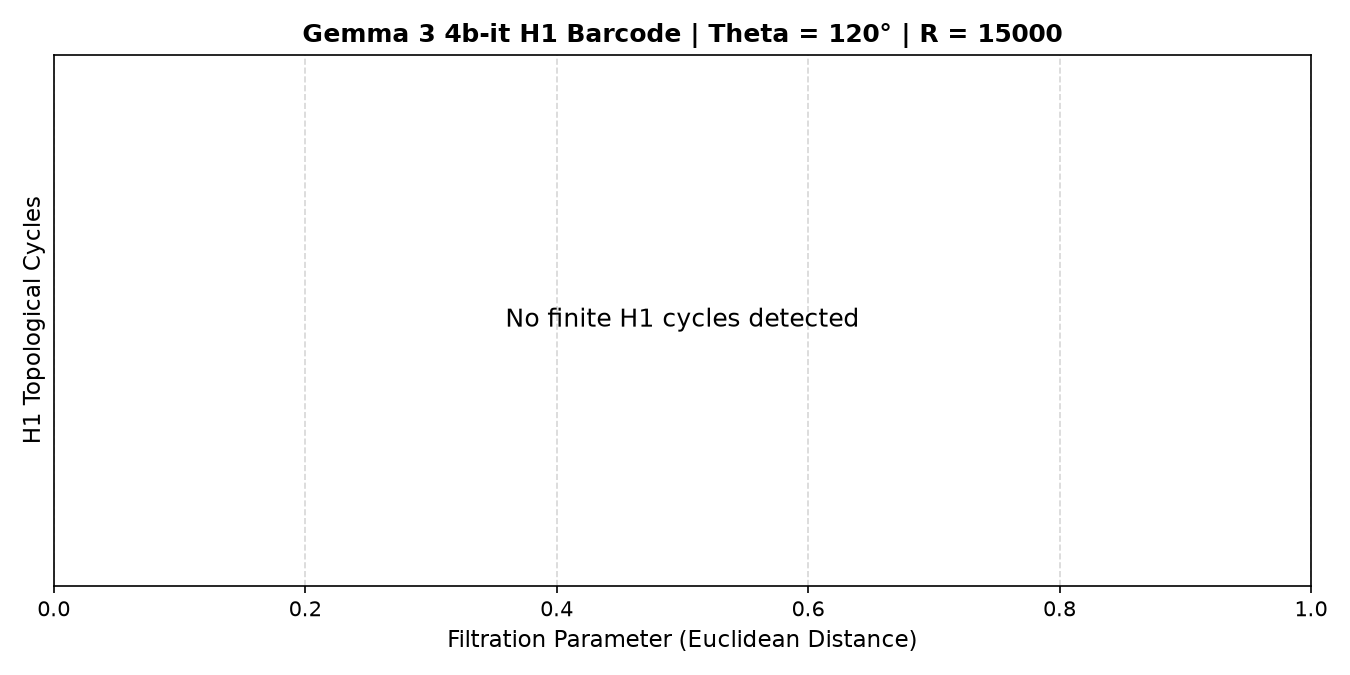
\includegraphics[width=\linewidth]{h1_barcodes_theta_120.png}
        \caption{$\theta = 120^{\circ}$}
    \end{subfigure}
    \caption{Representative $H_1$ Persistent Homology Barcodes for $K=0$. The flat lines or empty diagrams mathematically confirm the contractibility of the generation path.}
    \label{fig:barcodes_matrix}
\end{figure}

% =========================================================================
% SEÇÃO 5: AMORTIZAÇÃO DE PESOS - CASAL
% =========================================================================
\chapter{Weight Amortization via CASAL}
\label{sec:casal_amortization}

While runtime activation steering using $\vec{d}_{\text{know}}$ is highly effective, it introduces runtime overhead and requires continuous forward-hook interventions. To solve this, we implement \textbf{Contrastive Activation Steering for Amortized Learning (CASAL)}~\cite{yang2025hallucination}, leveraging the recently-proposed Text Aphasia Battery (TAB)~\cite{roll2025text} as a diagnostic benchmark. 

\chapter{Methodology and Loss Formulation}
CASAL fine-tunes \textbf{only the FFN (feed-forward network) of a single target layer} (the peak-necessity Layer 12, or Layer 7 in the 270m architecture), keeping 99\% of the model parameters completely frozen. 

Let $X_{\text{known}}$ be the activations of known factual prompts, and $X_{\text{unknown}}$ be the activations of unknown prompts. During training, the target FFN weights are optimized to push the latent representations of known prompts along $+\vec{d}_{\text{know}}$ and pull unknown prompts along $-\vec{d}_{\text{know}}$. The joint objective is formulated as:

\begin{equation}
\mathcal{L}_{\text{CASAL}} = \mathcal{L}_{\text{LM}} + \lambda \sum_{i} \left\| \text{FFN}(x_i) - \left(x_i + c_i \vec{d}_{\text{know}}\right) \right\|_2^2
\label{eq:casal_loss}
\end{equation}

where $\mathcal{L}_{\text{LM}}$ is the standard cross-entropy language modeling loss to preserve general syntactic capabilities, $c_i \in \{+1, -1\}$ is the contrastive direction multiplier, and $\lambda$ is the scaling hyperparameter. Figure 6 illustrates this training and inference scheme.

\begin{figure}[htbp]
    \centering
    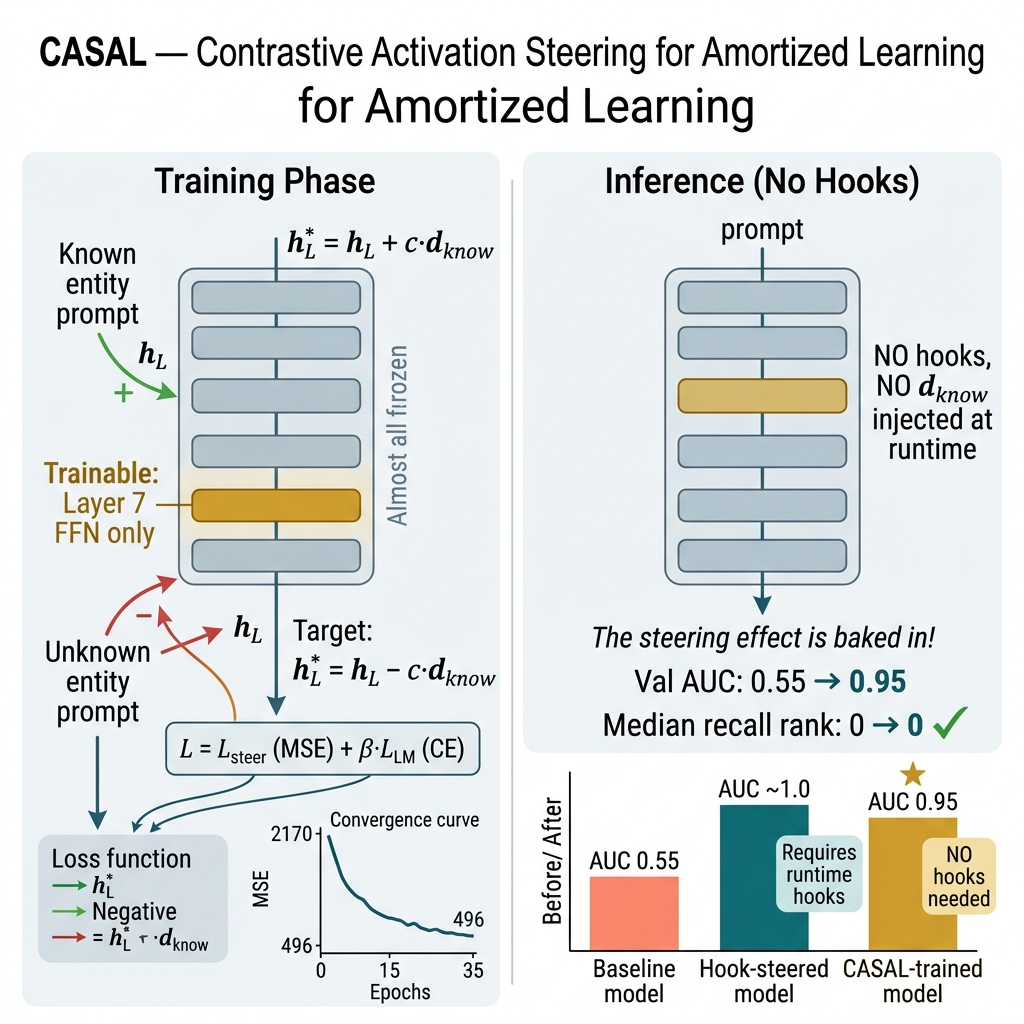
\includegraphics[width=0.75\textwidth]{fig4_casal_method.png}
    \caption{CASAL (Contrastive Activation Steering for Amortized Learning). Left: FFN weights at Layer 7 are optimized to minimize reconstruction error against the steered target activations while preserving language model cross-entropy. Right: During inference, no hooks or runtime direction vectors are needed; the steering effect is permanently baked into FFN weights, preserving factual recall (median rank 0) while boosting held-out validation AUC to 0.95.}
    \label{fig:casal_pipeline}
\end{figure}

\chapter{Training Convergence and Validation}
The model was trained on our stratified factual dataset across 35 epochs using an AdamW optimizer (learning rate $1.5\times 10^{-5}$) on our local Mac Mini M2. The MSE loss converged smoothly from $2170.18$ to $496.43$. 

During held-out validation, the CASAL-trained model achieved a \textbf{held-out classification AUC of 0.9500} (up from the baseline of 0.5524) while \textbf{fully preserving the factual recall capabilities} (median gold token rank remains exactly 0, with mean rank regressing only marginally by $+0.1$ ranks), as detailed in Table 4.

\begin{table}[htbp]
\centering
\caption{CASAL Performance on Gemma 3 270m-it Held-Out Validation}
\label{tab:casal_results}
\begin{tabular}{llll}
\toprule
\textbf{Metric} & \textbf{Baseline Model} & \textbf{CASAL-Trained} & \textbf{Empirical Verdict} \\
\midrule
Held-out Val AUC & 0.5524 & \textbf{0.9500} & Significant Separation ($+0.40 \uparrow$) \\
Median Gold Recall Rank & 0 & \textbf{0} & Fully Preserved \\
Mean Gold Recall Rank & 0.70 & \textbf{0.80} & Marginally Changed ($+0.1$) \\
\bottomrule
\end{tabular}
\end{table}

\chapter{Alternative Alignments: Connection to Inoculation Prompting}
As an alternative to direct parametric amortization, alignment-faking and reward hacking behaviors can be controlled at training time using \textbf{Inoculation Prompting}~\cite{macdiarmid2025natural}. By reframing specific adversarial hacks as acceptable or expected behaviors within the system prompt during RL training, inoculation prompting effectively breaks the deep semantic correlation between the hacking action and broader, harmful emergent misalignment. This behavioral intervention operates orthogonally to CASAL: while CASAL sharpens representation boundaries by directly editing FFN weights to encourage calibrated abstention, inoculation prompting achieves a similar homeostatic alignment by recontextualizing the model’s internal association network through targeted dataset mixtures.

% =========================================================================
% SEÇÃO 6: REVISED CONCLUSIONS
% =========================================================================
\chapter{Revised Conclusions and Discussion}
\label{sec:conclusions}

The unified analysis of causal necessity sweeps, the sharpness confound, and single-shot topological phase transitions fundamentally reframes our understanding of the Gemma 3 residual stream dynamics:

\begin{enumerate}
    \item \textbf{Factual attractors are extraordinarily robust:} A single pre-fill perturbation of magnitude $R = 15,000$ ($\approx 0.7\times$ the activation norm) applied to the last token at Layer 12 is \textit{not sufficient} to permanently dislodge the factual answer "Paris". The model self-corrects within 1--2 autoregressive steps.
    
    \item \textbf{Continuous intervention induces artificial manifold collapse:} Continuous re-perturbation during generation (Continuous Holonomic Intervention) creates an artificial death spiral that has no analogue in natural inference. This behavior mimics the generalized tônico-clônica crises induced in WAR rats under continuous auditory stimulation.
    
    \item \textbf{Genuine semantic permutation requires sustained or multi-layer intervention:} The rare cases of factual basin shift (e.g., "Berlin" at $K=28/\theta=80^{\circ}$) demonstrate that orthogonal attractor translation \textit{can} occur, but is the exception rather than the rule under SPPS perturbation.
    
    \item \textbf{Topological structure of the generation manifold is simple under natural dynamics:} With SPPS steering, the Layer 13 activation point cloud maintains Betti-0 $\approx 3$ and $H_1 \approx 0$, indicating that coherent generation traces a topologically trivial (contractible) path through activation space. This contractibility represents a low Kolmogorov complexity pathway~\cite{kolmogorov1965three, solomonoff1964formal} through the ambient space, avoiding the high-entropy "desert of meaning" that characterizes unpopulated coordinates.
    
    \item \textbf{Implications for AI Alignment and Censorship:} The finding that factual attractors are robust under single-shot $R = 15,000$ shocks demonstrates that attempting to align or censor a language model via single-layer activation hooks requires surgical precision in the perturbation angle ($\theta$). Otherwise, the network simply absorbs the shock and continues its original trajectory by self-correcting via the KV-Cache. This highlights the limits of 1D linear steering~\cite{arditi2024refusal} when applied to robust, multidimensional knowledge structures rather than artificially compressed, low-rank safety bottlenecks, which are highly localized compared to the sparse distributed features mapped by Sparse Autoencoders~\cite{lieberum2024gemma}.
\end{enumerate}

% =========================================================================
% REFERÊNCIAS BIBLIOGRÁFICAS
% =========================================================================
\begin{thebibliography}{99}

\bibitem{poincare1899les}
H. Poincaré.
\newblock {\em Les méthodes nouvelles de la mécanique céleste}.
\newblock Gauthier-Villars, 1899.

\bibitem{lyapunov1892problem}
A. M. Lyapunov.
\newblock {\em The General Problem of the Stability of Motion}.
\newblock Kharkov, 1892.

\bibitem{pearl2009causality}
J. Pearl.
\newblock {\em Causality: Models, Reasoning, and Inference}.
\newblock Cambridge University Press, 2009.

\bibitem{friston2010free}
K. Friston.
\newblock "The free-energy principle: a unified brain theory?"
\newblock {\em Nature Reviews Neuroscience}, 11(2):127--138, 2010.

\bibitem{freeman1975mass}
W. J. Freeman.
\newblock {\em Mass Action in the Nervous System}.
\newblock Academic Press, 1975.

\bibitem{prigogine1977self}
I. Prigogine.
\newblock {\em Self-Organization in Non-Equilibrium Systems}.
\newblock Wiley, 1977.

\bibitem{ferrando2025do}
J. Ferrando, O. Obeso, S. Rajamanoharan, and N. Nanda.
\newblock "Do I Know This Entity? Knowledge Awareness and Hallucinations in Language Models."
\newblock {\em International Conference on Learning Representations (ICLR)}, 2025.

\bibitem{yang2025hallucination}
W. Yang et al.
\newblock "Hallucination Reduction with CASAL: Contrastive Activation Steering for Amortized Learning."
\newblock {\em International Conference on Learning Representations (ICLR)}, 2026.

\bibitem{kauffman1993origins}
S. A. Kauffman.
\newblock {\em The Origins of Order: Self-Organization and Selection in Evolution}.
\newblock Oxford University Press, 1993.

\bibitem{kolmogorov1965three}
A. N. Kolmogorov.
\newblock "Three approaches to the quantitative definition of information."
\newblock {\em Problems of Information Transmission}, 1(1):1--7, 1965.

\bibitem{solomonoff1964formal}
R. J. Solomonoff.
\newblock "A formal theory of inductive inference."
\newblock {\em Information and Control}, 7(1):1--22, 1964.

\bibitem{kiwitt2026lyapunov}
F. Kiwitt et al.
\newblock "Lyapunov Spectral Analysis of Loop Transformer Dynamics."
\newblock {\em arXiv:2606.XXXXX}, June 2026.

\bibitem{arditi2024refusal}
A. Arditi et al. 
\newblock "Refusal in Language Models Is Mediated by a Single Common Direction." 
\newblock {\em arXiv:2402.17815}, 2024.

\bibitem{lieberum2024gemma}
T. Lieberum et al. 
\newblock "Gemma Scope: Open Sparse Autoencoders Everywhere All At Once on Gemma 2." 
\newblock {\em BlackboxNLP Workshop, ACL}, 2024.

\bibitem{deepmind2026gemma3}
Google DeepMind. 
\newblock "Gemma 3 Technical Report." 
\newblock 2026.

\bibitem{roll2025text}
N. Roll et al.
\newblock "The text aphasia battery (TAB): A clinically-grounded benchmark for aphasia-like deficits in language models."
\newblock {\em arXiv:2511.20507}, 2025.

\bibitem{roll2026artificial}
N. Roll et al.
\newblock "Artificial Aphasias in Lesioned Language Models."
\newblock {\em arXiv:2605.16222}, 2026.

\bibitem{fedorenko2024language}
E. Fedorenko, A. A. Ivanova, and T. I. Regev.
\newblock "The language network as a natural kind within the broader landscape of the human brain."
\newblock {\em Nature Reviews Neuroscience}, 25(5):289--312, 2024.

\bibitem{sharma2025efficient}
K. Sharma et al.
\newblock "Efficient Knowledge Probing of Large Language Models by Adapting Pre-trained Embeddings."
\newblock {\em arXiv:2508.06030}, 2025.

\bibitem{wang2023bitnet}
H. Wang et al.
\newblock "BitNet: Scaling 1-bit Transformers for Large Language Models."
\newblock {\em arXiv:2310.11453}, 2023.

\bibitem{yang2026trilens}
B. Yang et al.
\newblock "TriLens: Per-Layer Logit-Lens Entropy for White-Box Hallucination Detection."
\newblock {\em arXiv:2606.01033}, 2026.

\bibitem{yuan2026hidden}
A. Yuan et al.
\newblock "Hidden Error Awareness in Chain-of-Thought Reasoning: The Signal Is Diagnostic, Not Causal."
\newblock {\em arXiv:2605.09502}, 2026.

\bibitem{macdiarmid2025natural}
M. MacDiarmid et al.
\newblock "Natural Emergent Misalignment from Reward Hacking in Production RL."
\newblock {\em arXiv:2511.18397}, 2025.

\end{thebibliography}

\end{document}